% ============================================================
\section{Phương pháp StatLM}
% ============================================================
StatLM được thiết kế theo kiến trúc encoder--decoder ba tầng (Hình~\ref{fig:arch}).
Mỗi văn bản thô lần lượt đi qua hai tầng encoder thống kê (tóm tắt, trích xuất
keyphrase); tập keyphrase của tất cả văn bản sau đó được chuyển tới tầng decoder,
nơi LLM thực hiện phân cụm, đặt tên và gán nhãn. Đầu ra là một không gian nhãn
(các chủ đề có tên tiếng Việt) cùng danh sách nhãn cho mỗi văn bản. Pipeline hỗ
trợ xử lý tăng dần (incremental), bảo đảm tính thế giới mở (open-world).

Mặc dù pipeline có sử dụng các mô hình giám sát không phụ thuộc tác vụ
(task-agnostic) như bộ gán nhãn từ loại và các embedding tiền huấn luyện cho xử
lý ngôn ngữ nền tảng, tác vụ cốt lõi -- khám phá không gian nhãn và phân loại --
được thực hiện hoàn toàn theo hướng zero-shot, không dùng dữ liệu huấn luyện
theo miền.

\begin{figure*}[!t]
\centering
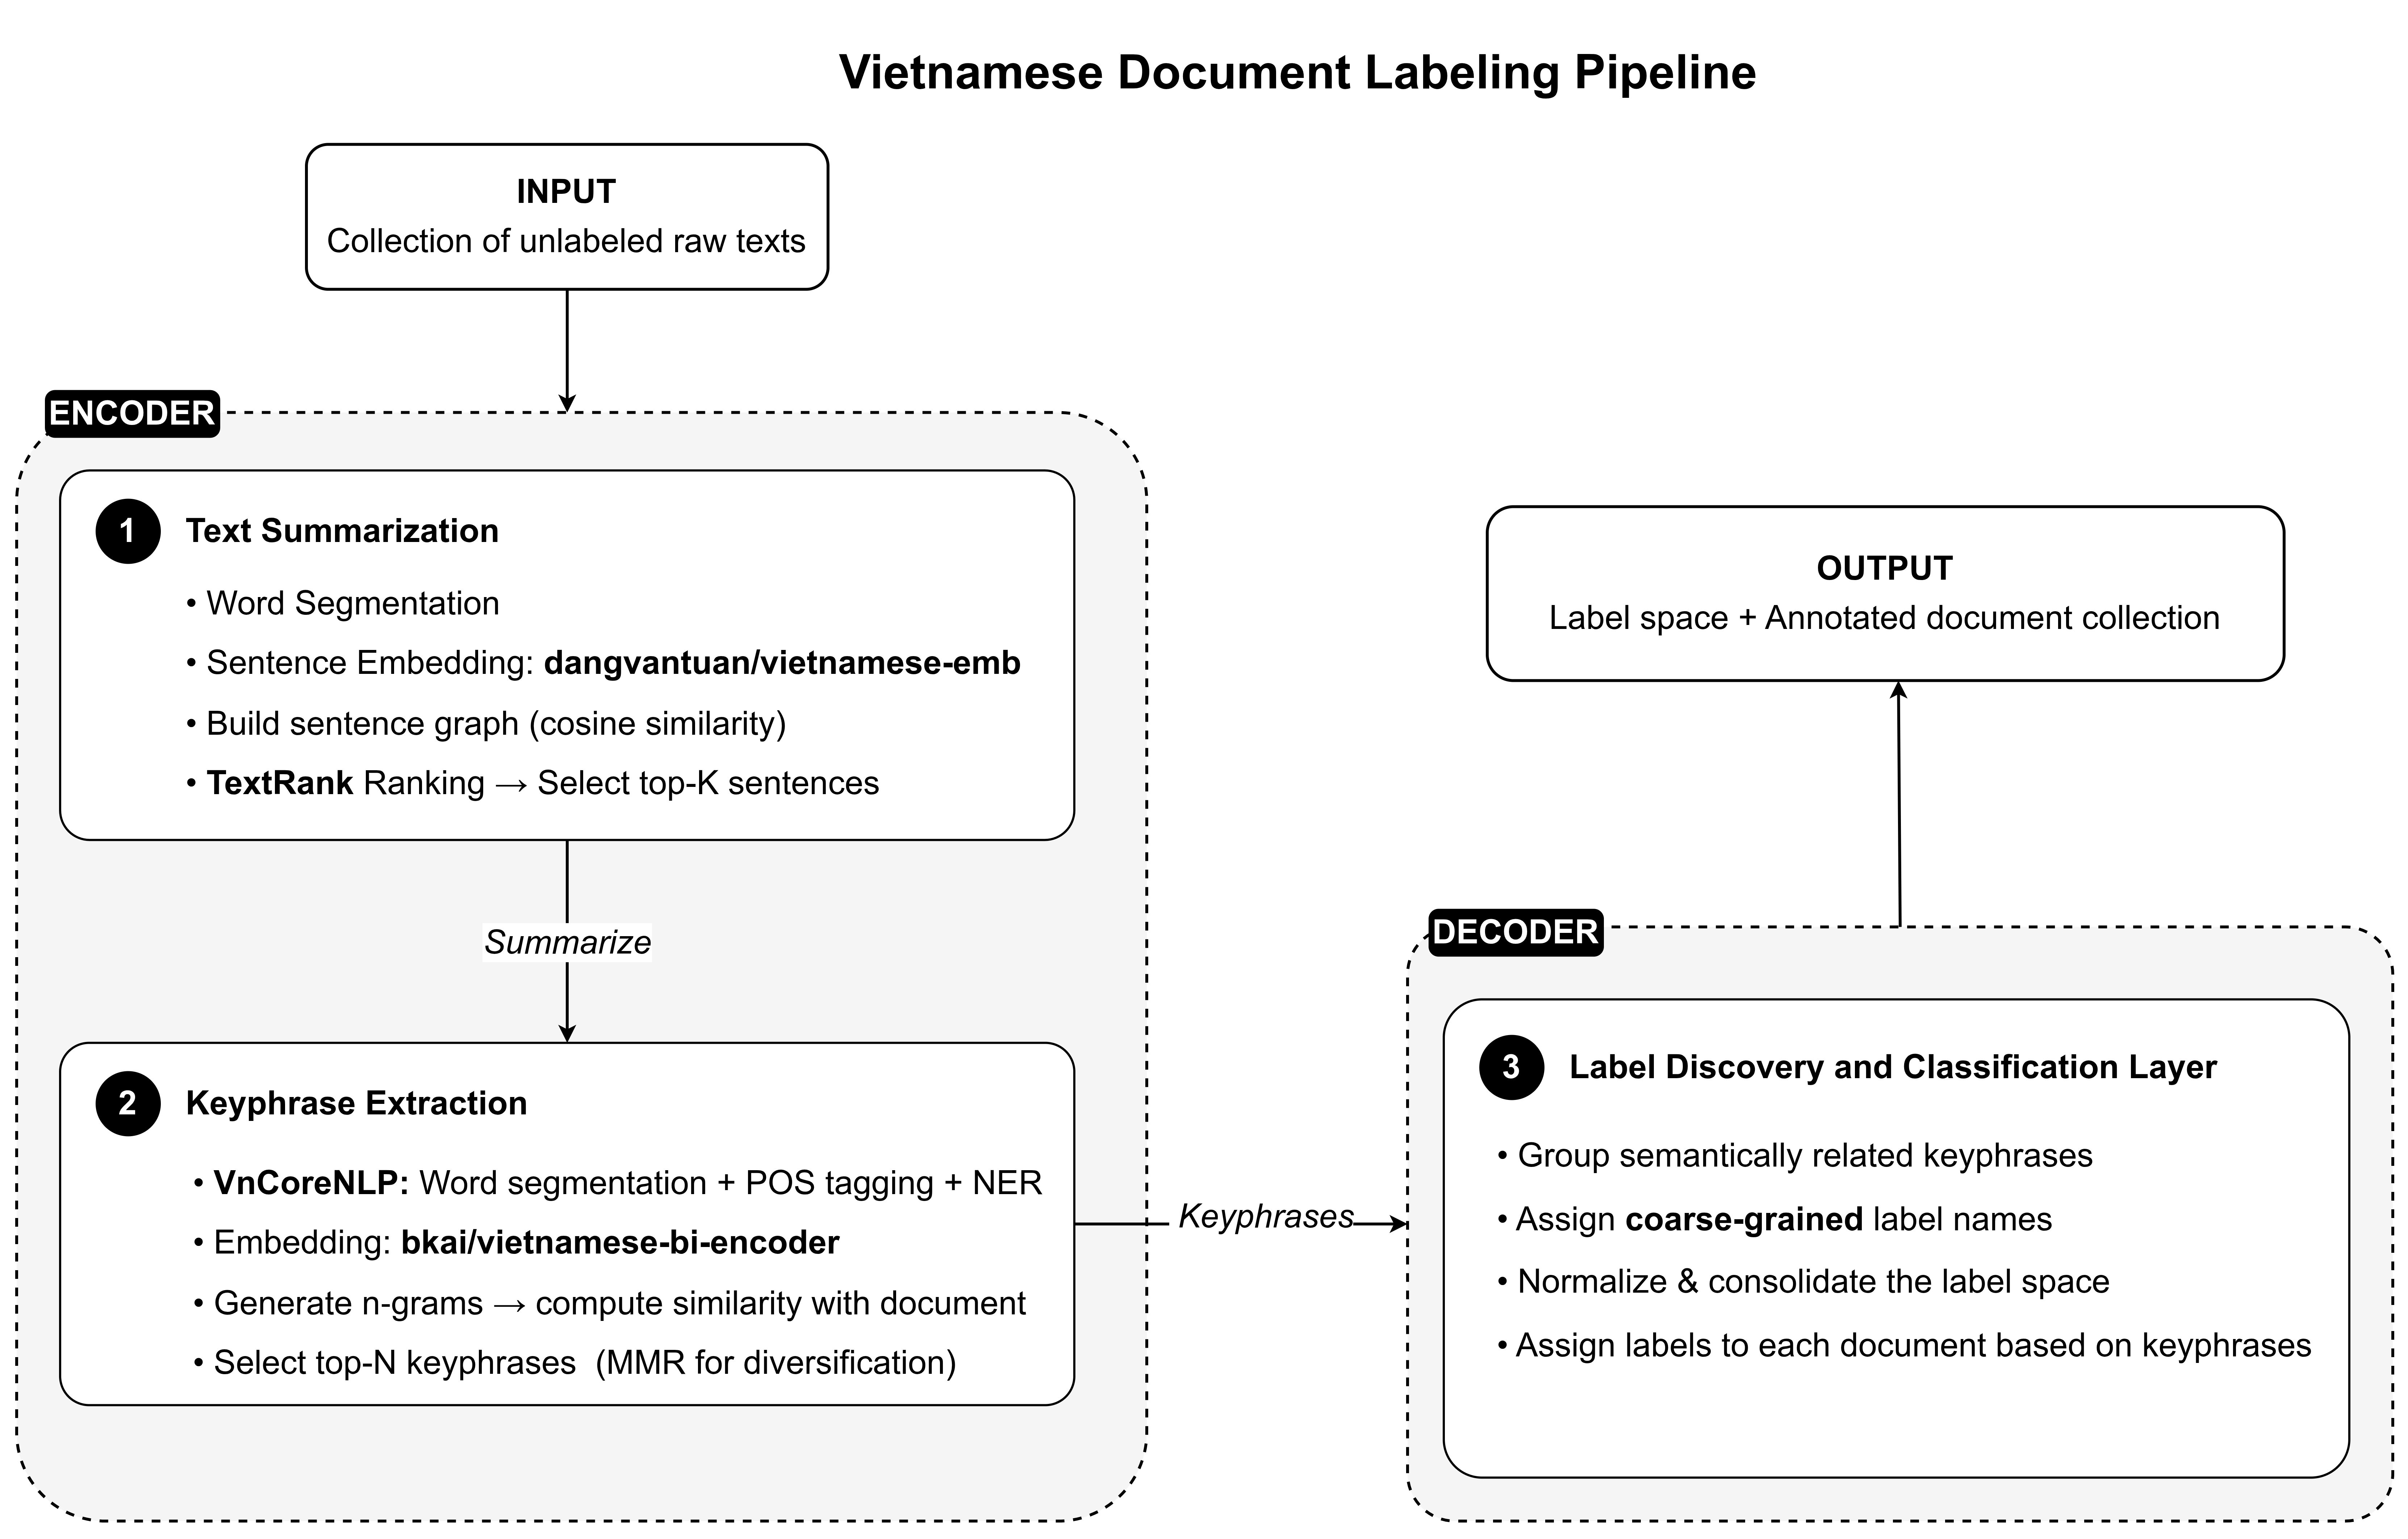
\includegraphics[width=0.95\textwidth]{figures/overview.png}
\caption{Kiến trúc tổng thể của StatLM: encoder thống kê gồm hai tầng (tóm tắt
văn bản với TextRank + \emph{dangvantuan/vietnamese-embedding}; trích xuất
keyphrase với KeyBERT + \emph{bkai/vietnamese-bi-encoder} và VnCoreNLP) làm nhiệm
vụ giảm nhiễu, cô đặc thông tin; decoder LLM (Gemini) chỉ được gọi một lần ở cuối
để khám phá, đặt tên và chuẩn hóa không gian nhãn rồi gán nhãn cho từng văn bản.}
\label{fig:arch}
\end{figure*}

\subsection{Tầng 1 -- Tóm tắt văn bản}
\textbf{Mục tiêu:} từ văn bản thô $D=\{s_1,\dots,s_n\}$ gồm $n$ câu, sinh bản tóm
tắt $S=\{s'_1,\dots,s'_k\}$ ($k<n$) nhằm loại bỏ câu ít quan trọng, tập trung vào
nội dung cốt lõi làm đầu vào cho Tầng~2.

Dựa trên phân tích ở Mục~\ref{sec:related}, StatLM chọn tóm tắt trích xuất dựa trên đồ thị câu
với thuật toán xếp hạng TextRank (PageRank cho hiệu suất tốt nhất và ổn định nhất
trong các độ đo trung tâm~\cite{kadriu2021extractive}). Điểm khác biệt then chốt
nằm ở \emph{hàm đo độ tương đồng}: thay vì Word Overlap, TF-IDF, BM25+ hay LDA
(đều chỉ phản ánh từ vựng bề mặt hoặc quá cồng kềnh), StatLM thực hiện bước nhảy
từ tương đồng từ vựng lên \emph{tương đồng ngữ nghĩa} bằng sentence embedding.
Bài toán ở đây có bản chất Semantic Textual Similarity \emph{đối xứng} (câu so
với câu, độ dài tương đương), nên StatLM dùng mô hình
\emph{dangvantuan/vietnamese-embedding}~\cite{dangvantuan2021vietnamese} cùng công
cụ tách từ pyvi để bảo đảm nhất quán giữa huấn luyện và suy luận.

Quy trình gồm năm bước: (1) tách câu bằng biểu thức chính quy, tách từ bằng pyvi;
(2) mã hóa mỗi câu thành vector $\mathbf{e}_i=\mathrm{meanpool}(\mathrm{PhoBERT}
(s_i))\in\mathbb{R}^{768}$; (3) xây đồ thị đầy đủ có trọng số với
$W_{ij}=\cos(\mathbf{e}_i,\mathbf{e}_j)$; (4) xếp hạng câu bằng TextRank với hệ số
giảm chấn $d=0{,}85$, ngưỡng hội tụ $\varepsilon=10^{-5}$ theo công thức cập nhật
\begin{equation}
\mathrm{WS}(v_i)^{(t+1)} = (1-d) + d\!\!\sum_{v_j\in \mathrm{In}(v_i)}
\frac{w_{ji}}{\sum_{v_k\in \mathrm{Out}(v_j)} w_{jk}}\,\mathrm{WS}(v_j)^{(t)};
\label{eq:textrank}
\end{equation}
(5) chọn $k$ câu điểm cao nhất ($k=\max(5,\lceil 0{,}4n\rceil)$ khi $n>5$) và sắp
xếp lại theo thứ tự gốc để bảo toàn mạch lạc. Hình~\ref{fig:textrank} minh họa đồ
thị câu đầy đủ có trọng số cùng bước xếp hạng của Tầng~1.

\begin{figure}[!t]
\centering
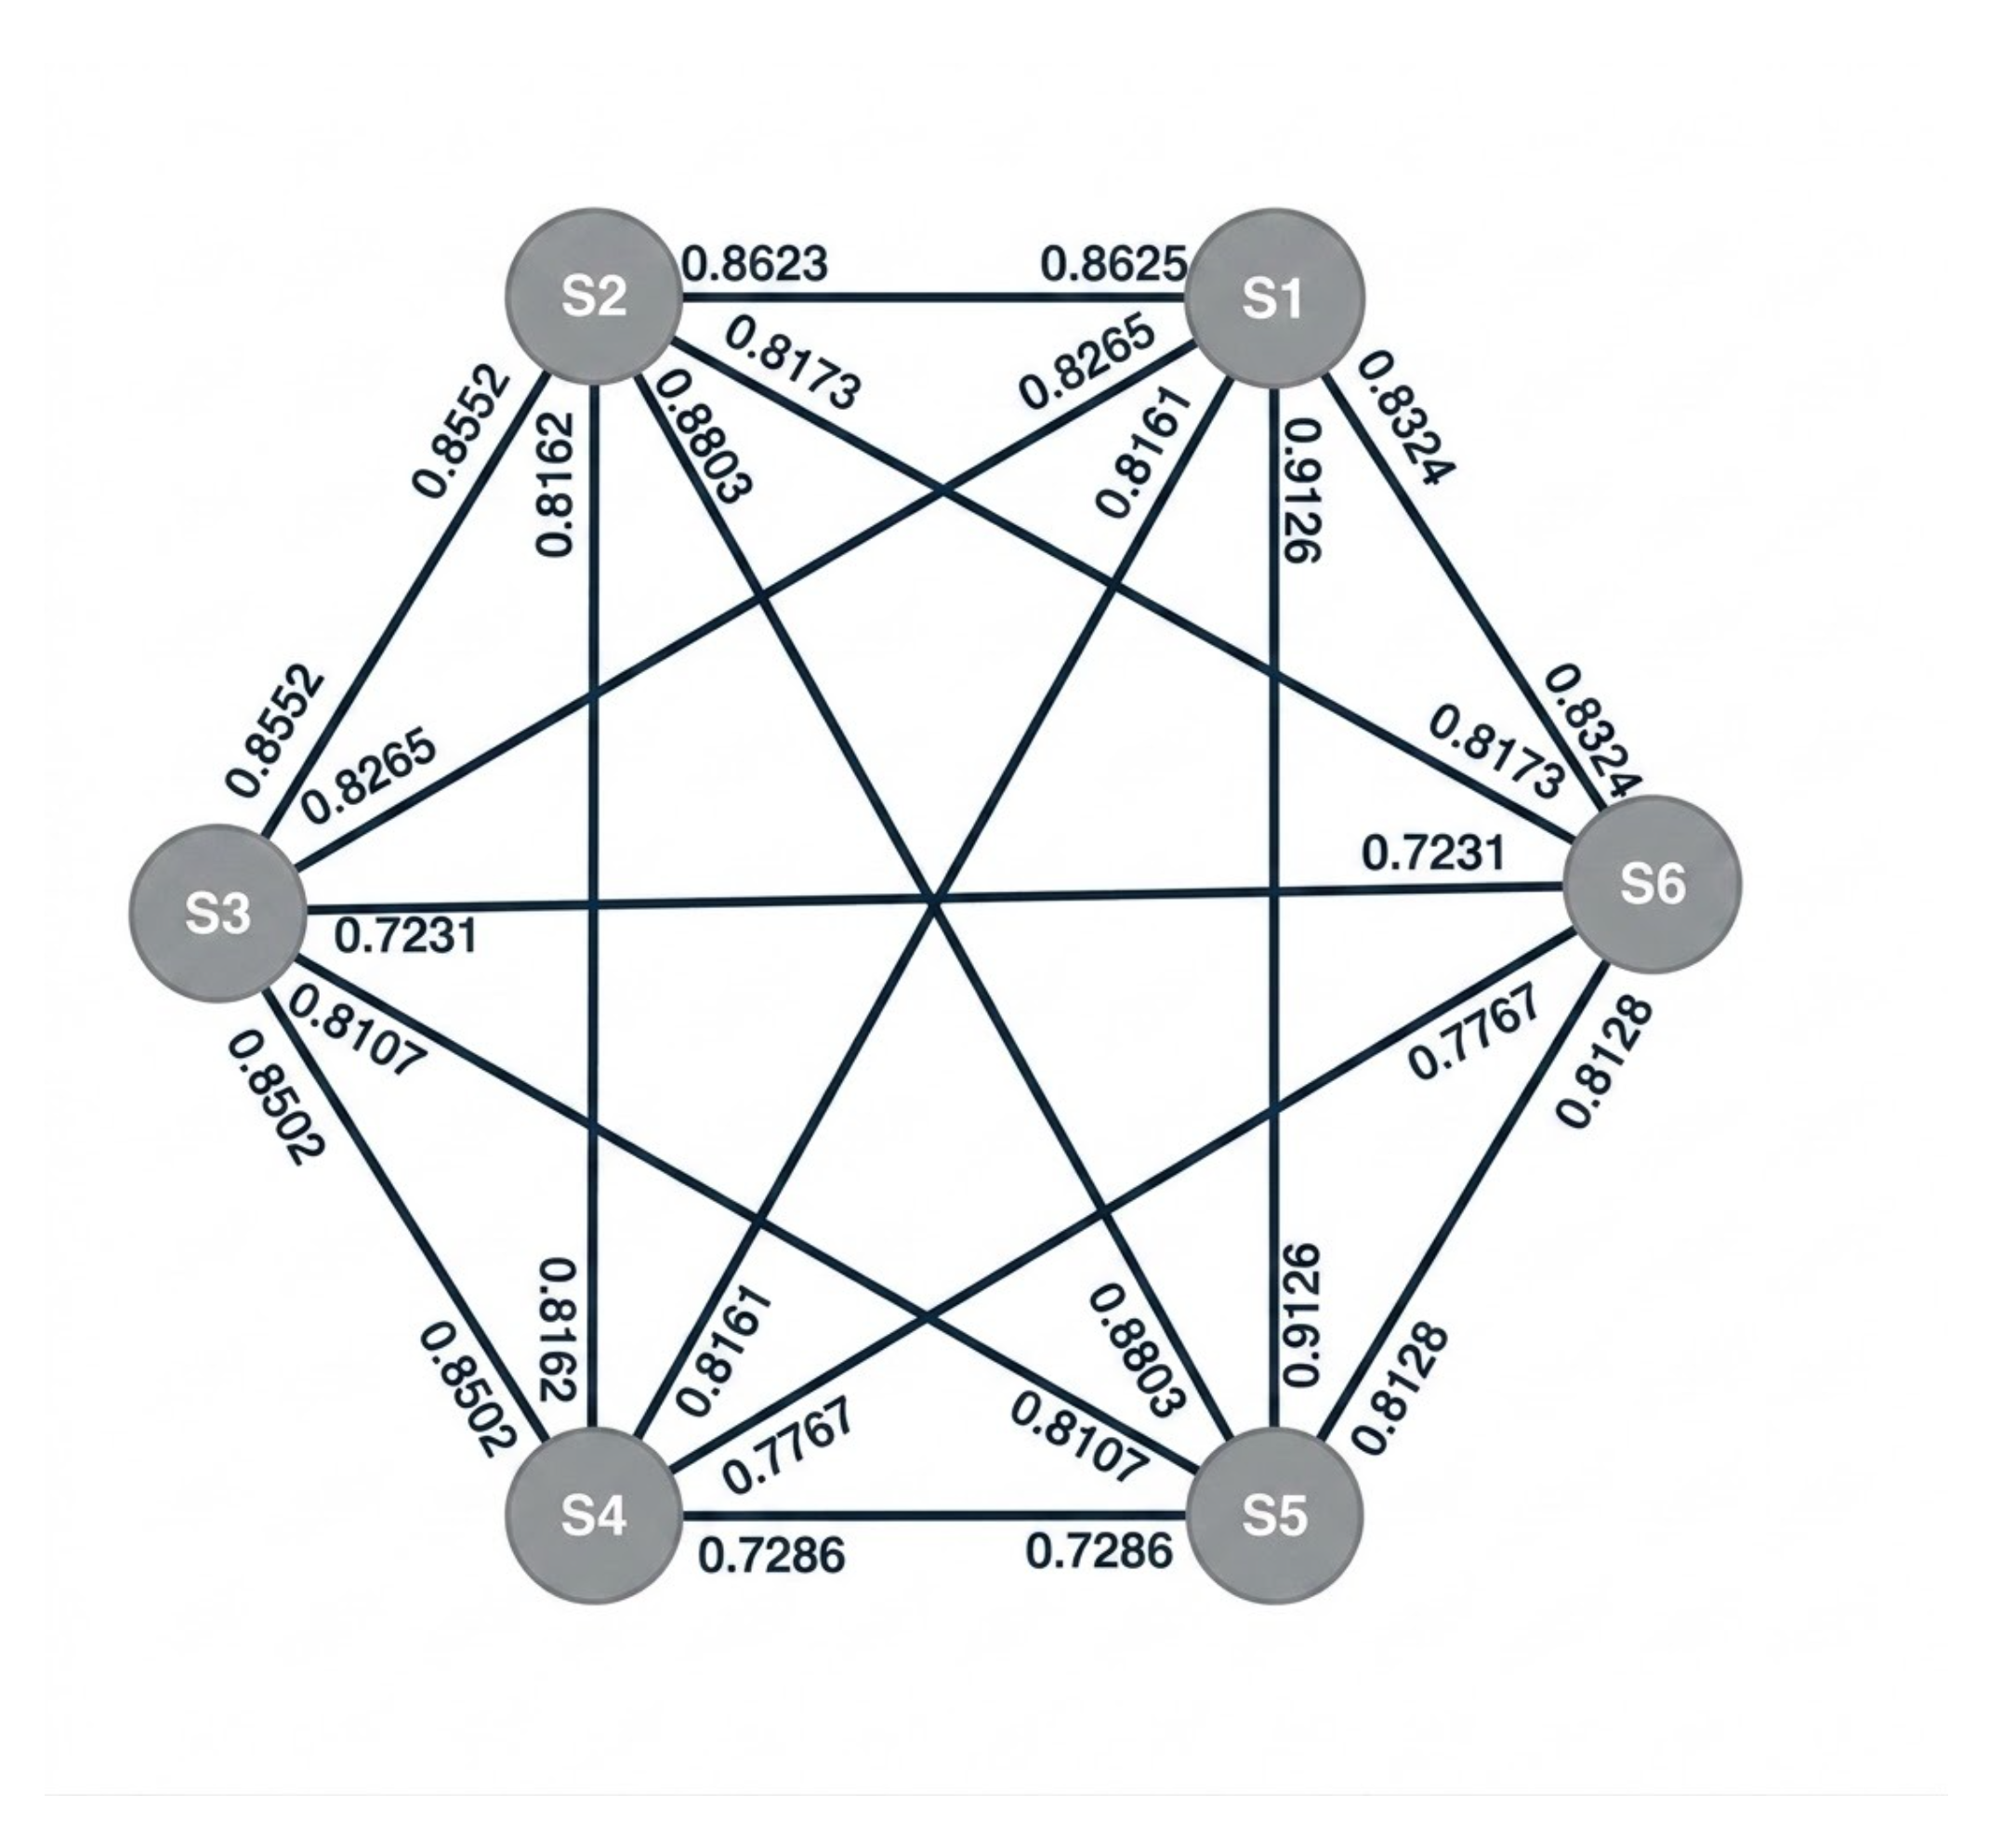
\includegraphics[width=0.92\columnwidth]{figures/stage1.png}
\caption{Đồ thị câu đầy đủ có trọng số ở Tầng~1: mỗi nút là một câu, trọng số
cạnh là độ tương đồng cosine giữa hai sentence embedding
(\emph{dangvantuan/vietnamese-embedding}); TextRank (PageRank) xếp hạng các nút và
chọn top-$k$ câu làm bản tóm tắt.}
\label{fig:textrank}
\end{figure}

\textbf{Về hệ số giảm chấn.} Chúng tôi cố định $d=0{,}85$ thay vì tinh chỉnh: đây
là giá trị kinh điển của PageRank~\cite{brin1998anatomy} và TextRank
gốc~\cite{mihalcea2004textrank}, và số hạng ``dịch chuyển'' $(1-d)$ trong
Eq.~\eqref{eq:textrank} chỉ để bảo đảm bước đi ngẫu nhiên ergodic, không mã hóa
thiên lệch theo ngữ liệu, nên \emph{thứ hạng} câu---và phép chọn top-$k$ mà Tầng~1
dùng---được ghi nhận là ổn định với $d$ trong dải chuẩn $[0{,}8;0{,}9]$. Chúng tôi
cũng tránh hướng ngược lại là hệ số giảm chấn \emph{động}: Extended TextRank của Vora
và cộng sự~\cite{vora2024extractive} kết hợp điểm LDA toàn cục và tính $d$ theo từng
tài liệu, nhưng chi phí LDA cùng trọng số kết hợp phải tinh chỉnh theo từng bộ dữ
liệu (ví dụ $0{,}1$ cho CNN/DailyMail so với $0{,}8$ cho BBC) đưa trở lại đúng kiểu
hiệu chỉnh bán giám sát mà StatLM muốn tránh. Việc cố định $d=0{,}85$ vì thế giữ
Tầng~1 không giám sát, để lại ngân sách giữ câu $r$ (bên dưới) là tham số Tầng~1 duy
nhất tương tác với dữ liệu.

\textbf{Về các câu bị bỏ.} Một câu bị \emph{loại bỏ} khi điểm TextRank
$\mathrm{WS}(s_i)$ trong Eq.~\eqref{eq:textrank} nằm ngoài nhóm top-$k$; do điểm này
tích lũy độ tương đồng ngữ nghĩa có trọng số giữa câu với toàn bộ văn bản, khoảng
$60\%$ câu bị loại là các nút có độ trung tâm thấp---câu diễn đạt lại dư thừa, câu
chuyển ý, câu khuôn mẫu và những câu lề liên kết yếu với lõi văn bản. Một chủ đề
chính được nhắc lại qua nhiều câu và gần như không bao giờ bị mất, trong khi một chủ
đề phụ chỉ hiện diện ở vài câu có độ trung tâm thấp có thể rơi dưới ngưỡng cắt và,
vì pipeline là vòng hở, không thể khôi phục ở các tầng sau. Tỉ lệ giữ lại được chọn
theo thực nghiệm: quét $r\in[0{,}2;0{,}6]$ (Bảng~\ref{tab:retention}) cho thấy độ gần
lõi tiêu đề+sapo giảm theo $r$ còn độ phủ chủ đề tăng, nên chúng tôi lấy mốc vận hành
$40\%$. Việc đặt ngân sách theo \emph{tỉ lệ} ($k=\max(5,\lceil 0{,}4n\rceil)$) thay vì
lead-$k$ cố định cho các chủ đề phụ nằm cuối bài cơ hội tồn tại, nhất quán với việc
TextRank trên embedding vượt Lead-$K$ về ROUGE (Bảng~\ref{tab:rouge}).

\subsection{Tầng 2 -- Trích xuất cụm từ khóa}
\textbf{Mục tiêu:} từ bản tóm tắt $S$, trích $m$ keyphrase (mặc định $m=10$, mỗi
cụm 1--3 từ) đại diện các khía cạnh nội dung chính, làm đầu vào cho Tầng~3.

StatLM dùng KeyBERT~\cite{grootendorst2020keybert}. Khác với Tầng~1, bài toán
KeyBERT mang bản chất \emph{bất đối xứng} (keyphrase ngắn so với tài liệu dài),
nên một mô hình xuất sắc cho STS đối xứng không đương nhiên tối ưu ở đây. StatLM
do đó chọn mô hình embedding riêng cho Tầng~2:
\emph{bkai-foundation-models/vietnamese-bi-encoder}~\cite{nguyen2025improving},
vốn được huấn luyện cho truy xuất ``truy vấn ngắn $\rightarrow$ tài liệu dài''
(Legal Text Retrieval) -- trùng khớp với cơ chế của KeyBERT. Tầng~2 còn dùng
VnCoreNLP~\cite{vu2018vncorenlp} để gán nhãn từ loại (chỉ giữ danh từ, danh từ
riêng, động từ, tính từ làm ứng viên n-gram) và nhận dạng thực thể (bảo toàn thực
thể có tên).

Quy trình: (1) tiền xử lý bằng VnCoreNLP, lọc stopword và lọc theo từ loại; (2)
mã hóa văn bản tóm tắt thành $\mathbf{E}_{doc}$; (3) sinh tập n-gram ứng viên
(1--3 từ) trong từng mảnh câu, bổ sung các thực thể NER; (4) tính độ tương đồng
\begin{equation}
\cos(\mathbf{E}_{doc},\mathbf{E}_{ngram}) =
\frac{\mathbf{E}_{doc}\cdot \mathbf{E}_{ngram}}
{\lVert \mathbf{E}_{doc}\rVert\,\lVert \mathbf{E}_{ngram}\rVert};
\label{eq:cosine}
\end{equation}
(5) chọn keyphrase bằng MMR~\cite{carbonell1998use} để cân bằng độ liên quan và
tính đa dạng:
\begin{equation}
\mathrm{MMR} = \arg\max_{c\notin S}\Big[\lambda\,\mathrm{sim}(c,doc)
-(1-\lambda)\max_{s\in S}\mathrm{sim}(c,s)\Big],
\label{eq:mmr}
\end{equation}
với $\lambda=0{,}5$ và ngưỡng trùng lặp tối đa $\theta=0{,}7$.

\textbf{Về các tham số MMR.} Chúng tôi đặt $\lambda$ ở trung điểm trung tính $0{,}5$,
điểm cân bằng giữa thuần liên quan ($\lambda\!\to\!1$) và thuần đa dạng
($\lambda\!\to\!0$)~\cite{carbonell1998use}: tập 5 keyphrase gửi xuống Tầng~3 phải
cùng nhau \emph{bao phủ} các khía cạnh của văn bản, nên thiên về liên quan sẽ lấp
danh sách bằng các biến thể gần trùng của cụm trung tâm nhất, còn thiên về đa dạng
lại nạp những cụm liên quan lỏng lẻo trở thành nhiễu nhãn. Ngưỡng trùng lặp
$\theta=0{,}7$ là phần bổ trợ ``cứng'' cho hình phạt ``mềm'' nói trên---một ứng viên
bị loại khi cosine với một keyphrase đã chọn vượt $\theta$---được đặt thận trọng để
các khía cạnh khác biệt nhưng gần chủ đề vẫn được giữ trong khi loại các cụm gần đồng
nghĩa hay trùng thành phần. Vì ứng viên đã được lọc từ loại và NER, hai số hạng nằm
trên cùng thang cosine và việc chọn ổn định quanh $(\lambda,\theta)=(0{,}5;0{,}7)$.

Quy trình của Tầng~2 được minh họa trong Hình~\ref{fig:keybert}. Như thể hiện trong hình, văn
bản tóm tắt và tập n-gram ứng viên (được bổ sung các thực thể có tên) được mã hóa
độc lập bởi \emph{bkai/vietnamese-bi-encoder}, và ma trận tương đồng cosine giữa
chúng quyết định việc xếp hạng. Sau đó, MMR vận hành trên ma trận này để chọn ra
top-$k$ keyphrase đa dạng, phản ánh bản chất bất đối xứng của bài toán so khớp
(tài liệu dài so với keyphrase ngắn). Bảng~\ref{tab:emb} đối chiếu
hai mô hình embedding được dùng ở hai tầng -- minh họa nguyên lý ``mỗi tầng dùng
đúng loại embedding phù hợp với bản chất bài toán''.

\begin{figure*}[!t]
\centering
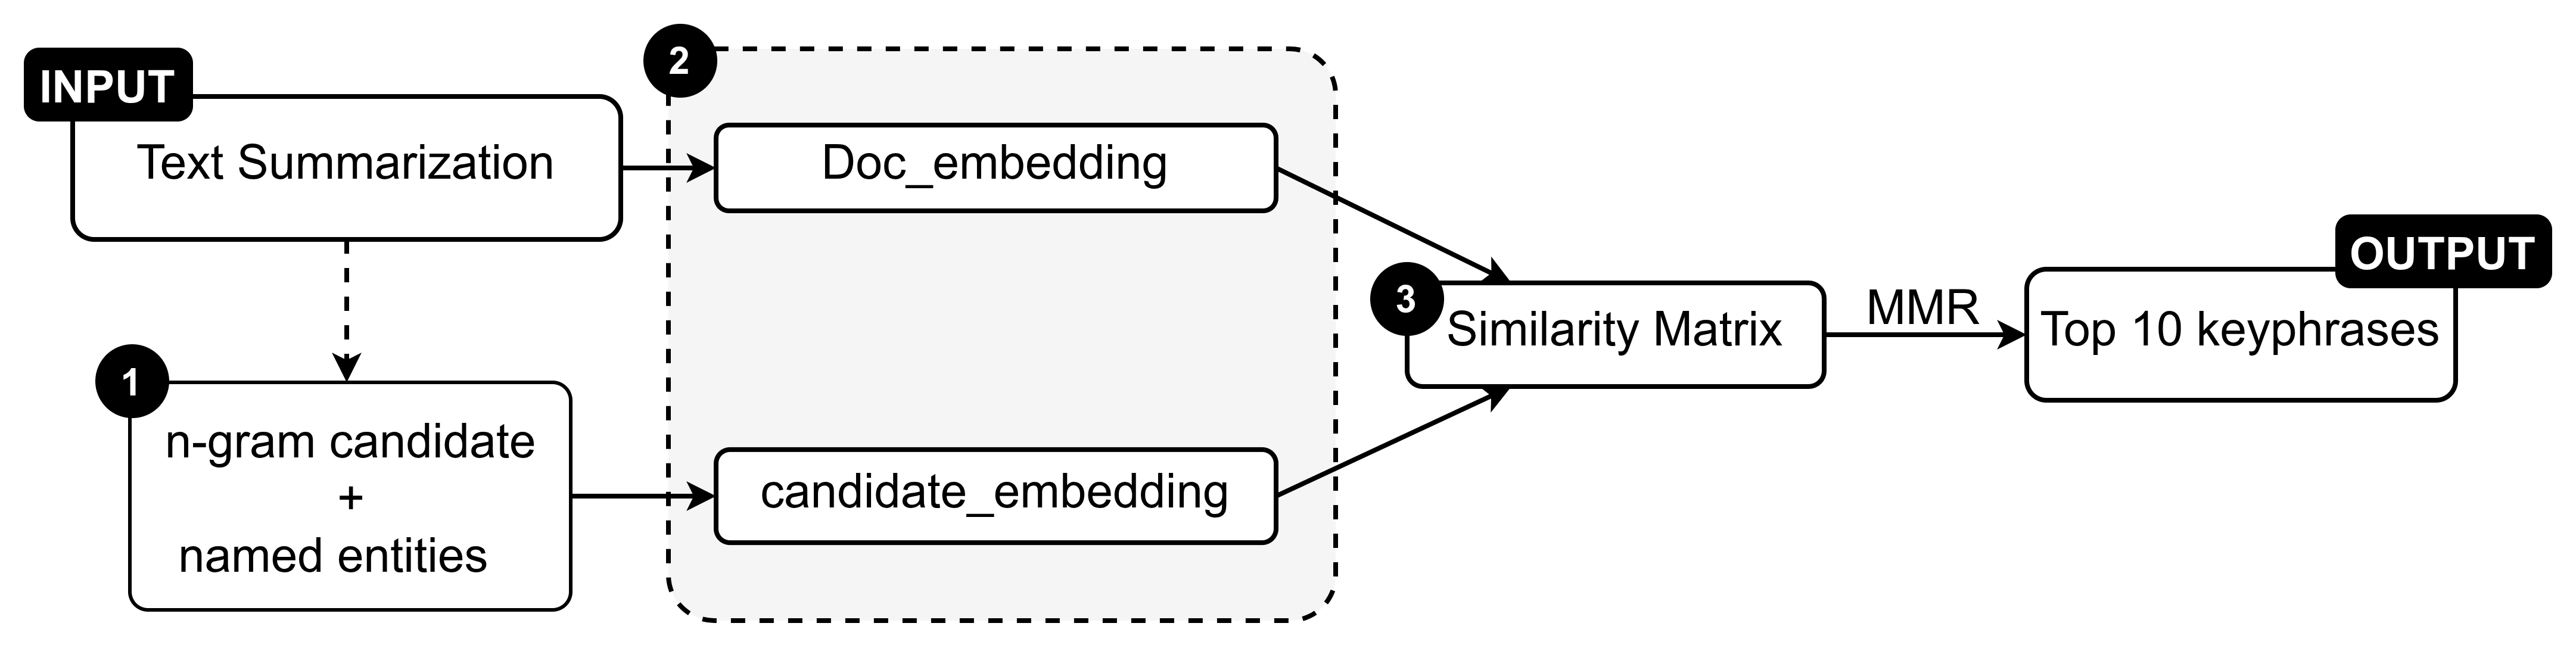
\includegraphics[width=0.95\textwidth]{figures/stage2.png}
\caption{Quy trình Tầng~2 (KeyBERT): văn bản tóm tắt và tập n-gram ứng viên (kèm
thực thể có tên) được mã hóa độc lập bằng \emph{bkai/vietnamese-bi-encoder}; ma
trận tương đồng cosine giữa chúng được dùng để xếp hạng, và MMR chọn ra top-$k$
keyphrase đa dạng. Đây là một bài toán bất đối xứng (tài liệu dài -- keyphrase
ngắn).}
\label{fig:keybert}
\end{figure*}

\begin{table}[!t]
\renewcommand{\arraystretch}{1.25}
\caption{Đối chiếu hai mô hình embedding trong StatLM}
\label{tab:emb}
\centering
\scriptsize
\begin{tabularx}{\columnwidth}{@{}lXX@{}}
\toprule
\textbf{Tiêu chí} & \textbf{Tầng 1 (TextRank)} & \textbf{Tầng 2 (KeyBERT)} \\
\midrule
Bài toán   & STS (đối xứng) & Truy xuất (bất đối xứng) \\
Quan hệ    & câu $\leftrightarrow$ câu & keyphrase ngắn $\leftrightarrow$ tài liệu dài \\
Mô hình    & dv-embedding & bkai-bi-encoder \\
Tách từ    & pyvi & VnCoreNLP \\
Đánh giá   & Pearson 84,21 & \#1 VCS retrieval \\
\bottomrule
\end{tabularx}
\end{table}

\subsection{Tầng 3 -- Phân loại và gán nhãn với LLM}
\textbf{Mục tiêu:} từ tập keyphrase $\mathcal{P}=\{p_1,\dots,p_N\}$ của $N$ văn
bản, tự động khám phá không gian nhãn $\mathcal{L}=\{l_1,\dots,l_M\}$ và gán nhãn
cho từng văn bản.

StatLM đặt LLM (Gemini 2.5 Flash) ở vị trí \emph{decoder} cuối pipeline, sau khi
dữ liệu đã được lọc và cô đặc. Cách thiết kế này giảm mạnh số token gửi đến API
(chỉ gửi keyphrase, không gửi văn bản thô) và hạn chế nhãn nhiễu (LLM không bị
phân tán bởi thực thể/định dạng trong văn bản gốc). Tầng~3 hoạt động theo ba bước, hỗ
trợ cả dữ liệu mới hoàn toàn lẫn dữ liệu bổ sung tăng dần: (1) với mỗi văn bản,
chỉ gửi tối đa 5 keyphrase điểm cao nhất để LLM chuẩn hóa; (2) gán văn bản vào các
cụm hiện có theo chiến lược ``nghiêm ngặt'', cho phép đề xuất đổi tên nhãn, đưa
văn bản không khớp vào danh sách ``chưa gán''; (3) phân cụm và đặt tên cho các văn
bản chưa gán. LLM được System Message hướng dẫn sinh nhãn ở mức khái quát
(coarse-grained), tránh nhãn quá chi tiết hay mang tính thực thể (ví dụ ``Giáo
dục'' thay vì ``Tuyển sinh đại học 2024''), đồng thời tối thiểu hóa số nhãn và
gộp các chủ đề tương đồng.

